%
% Copyright (c) 2011-2012, fortiss GmbH.
% Licensed under the Apache License, Version 2.0.
% 
% Use, modification and distribution are subject to the terms specified
% in the accompanying license file LICENSE.txt located at the root directory
% of this software distribution. A copy is available at
% http://chromosome.fortiss.org/.
%
% This file is part of CHROMOSOME.
%
% $Id$
%
% Author:
%         Dominik Sojer <sojer@fortiss.org>
%         Michael Geisinger <geisinger@fortiss.org>
%

\section{Example 2: Chat with Chat Rooms (30 minutes)}
\label{sec:example_chat}

It is now time to replace the \emph{Hello World} application with a distributed \emph{Chat} application.
This tutorial comes with components that realize a distributed chat service.
The source code of this application is already present in the tutorial project,
we just need to configure it properly.

\begin{enumerate}
	\item The \emph{Hello World} application was using a specific component to print its ``\texttt{Hello World!}'' message.
		As this message is quite annoying in a chat room, we first have to remove the \emph{Hello World} component from the tutorial project.
		At the same time, we enable the \emph{Chat Component} which implements the chat client.
		This has to be done in the project's main file {\tt tutorial.c},
		which can be opened in Visual Studio by double-clicking on the respective item
		below \emph{tutorial} $\rightarrow$ \emph{Source Files} in the \emph{Project Explorer} pane.
		Please comment the line with the {\tt helloWorldComponent}
		and uncommend (enable) the line with the {\tt chatComponent} as shown below:

\begin{lstlisting}[numbers=left,firstnumber=48]
/*************************************************************************/
/***   Component descriptor                                            ***/
/*************************************************************************/
XME_COMPONENT_LIST_BEGIN
	XME_COMPONENT_LIST_ITEM(xme_core_nodeManager, 0)
	XME_COMPONENT_LIST_ITEM(xme_prim_ipLoginServerProxy, 0)
/*	XME_COMPONENT_LIST_ITEM(helloWorldComponent, 0)*/ /~~/ Comment this line
	XME_COMPONENT_LIST_ITEM(chatComponent, 0)       /~~/ Uncomment this line
XME_COMPONENT_LIST_END;
\end{lstlisting}

	\item The routing of messages is performed automatically by \xme core components.
		To keep the tutorial project small, all required components for network management and routing messages
		between distributed nodes (i.e., \emph{Login Server} and \emph{Master Directory}) have been added to a separate project named {\bf Coordinator}.
		We will treat the Coordinator as a separate node and have it running in the background so that people can dynamically enter chat rooms.
		
		To be able to use this functionality, please go go back to Section~\ref{sec:example_helloworld}
		and perform the described steps again for the \verb|coordinator| example.
		Please use the directory \verb|<XME_ROOT>/| \verb|examples/coordinator| as input for the \emph{Where is the source code} field
		and use the directory \verb|<XME_ROOT>/examples/build/coordinator| as input for the
		\emph{Where to build the binaries} field within CMake.
		After generation of the build system, the \verb|Coordinator.sln| Visual Studio solution file
		can be found in at \verb|<XME_ROOT>/examples/build/coordinator|.
		Do not forget to set up \verb|coordinator| as the \emph{StartUp Project} within Visual Studio.
		
	\item After having successfully compiled the coordinator project as well as the tutorial project,
		a basic distributed chat application can be started.
		In order to do this, execute {\bf one instance} of the coordinator application.
		If you receive a request from the \emph{Windows Firewall},
		please allow communication to the \emph{Home or Company Network} as shown in Figure~\ref{fig:firewall_coordinator}.
		Note that if you have colleagues on the same network running this tutorial at the same time,
		you should talk to them to only run one instance of the Coordinator at any point in time.\footnote{%
			This is a limitation of the current version of \xme. We do not yet support multiple subnets
			or detect the presence of other Coordinator instances. This will change in future versions.}
		
		The Coordinator can either be started from Visual Studio or by executing \verb|<XME_ROOT>/|
		\verb|examples/build/coordinator/target/*/coordinator.exe|.
		This will open a terminal window in which \xme may print logging information.
		By default, the log level is set up so that only warnings and errors will be shown,
		so it is normal for the terminal window to not show any activity.

\begin{figure}[htpb]
	\centering
	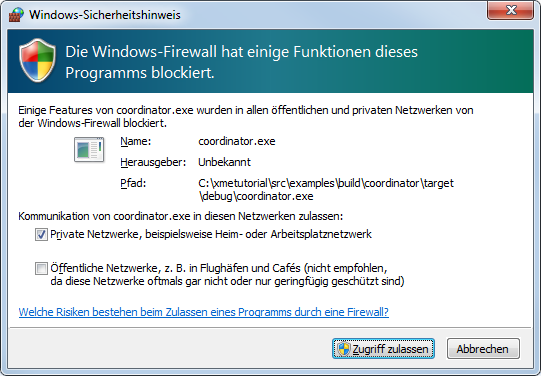
\includegraphics[scale=0.75]{figures/PNG/firewall_coordinator.png}
	\caption{Firewall settings for the \texttt{Coordinator} application.}
	\label{fig:firewall_coordinator}
\end{figure}

	\item We can now execute an arbitrary number of instances of the tutorial application.
		To do this, navigate to the respective directory and launch
		\verb|<XME_ROOT>/examples/build/| \verb|tutorial/target/*/tutorial.exe|.
		This will also open a terminal window, which first prompts to enter a name.
		After a name is given, you will be presented a list of commands and chat rooms to choose from
		(compare Figure~\ref{fig:example_chat}).

\begin{figure}[htpb]
	\centering
	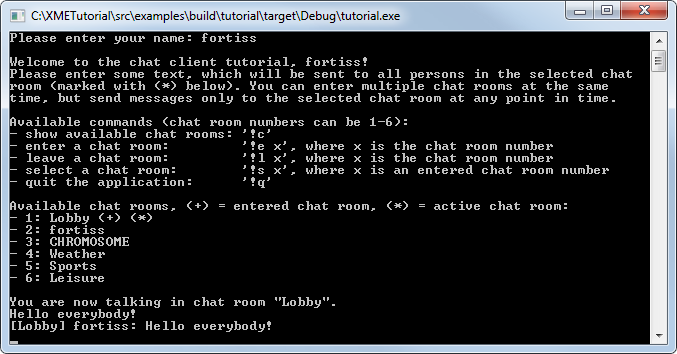
\includegraphics[scale=0.75]{figures/PNG/example_chat.png}
	\caption{Sending chat messages via the \emph{Chat Component}.}
	\label{fig:example_chat}
\end{figure}

		The semantics of a chat room are that messages sent to a chat room should only be visible to people that have joined the respective chat room.
		This concept can be directly mapped to the notion of \emph{topics}.
		
		Anything that is not a command is interpreted as a message to send to the \emph{active} chat room.
		The active chat room can be changed with the \texttt{!s} command.
		
		Launch multiple instances of the chat example using different names and send some messages.
		Then run the application in a distributed way using multiple computers on the same subnet.

\end{enumerate}
